\documentclass[tikz]{standalone}
\usepackage[utf8]{inputenc}

\usetikzlibrary{shapes.geometric, arrows}

\tikzstyle{startstop} = [rectangle, rounded corners, minimum width=3cm, minimum height=1cm,text centered, draw=black, fill=red!30]
\tikzstyle{io} = [trapezium, trapezium left angle=70, trapezium right angle=110, minimum width=3cm, minimum height=1cm, text centered, draw=black, fill=blue!30]
\tikzstyle{process} = [rectangle, minimum width=3cm, minimum height=1cm, text centered, text width=3cm, draw=black, fill=orange!30]
\tikzstyle{decision} = [diamond, minimum width=3cm, minimum height=1cm, text centered, draw=black, fill=green!30]
\tikzstyle{arrow} = [thick,-latex]

\begin{document}

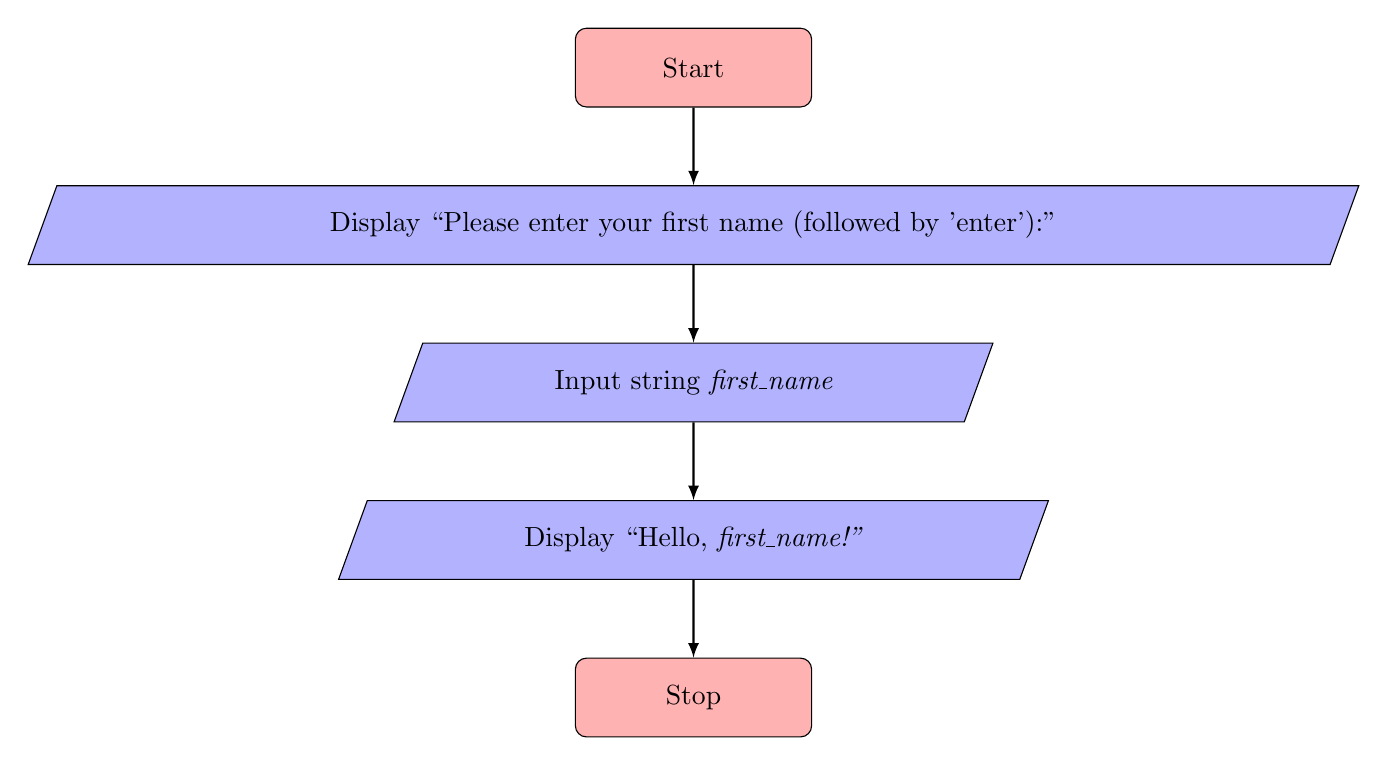
\begin{tikzpicture}[node distance=2cm]

\node (start) [startstop] {Start};
\node (out1) [io, below of=start] {Display ``Please enter your first name (followed by 'enter'):''};
\node (in) [io, below of=out1] {Input string \it{first\_name}};
\node (out2) [io, below of=in] {Display ``Hello, \it{first\_name}!''};
\node (stop) [startstop, below of=out2] {Stop};

\draw [arrow] (start) -- (out1);
\draw [arrow] (out1) -- (in);
\draw [arrow] (in) -- (out2);
\draw [arrow] (out2) -- (stop);

\end{tikzpicture}

\end{document}
